\subsection{Domainanalyse}

Das Domain-Modell besteht grob aus zwei Teilen: den Benutzern und der Brainstorming Methodik. 

Dabei bilden mehrere Participants ein \textit{Brainstorming Team}. Diese wird von einem der Participants, dem \textit{Moderator}, gegründet.  Das Team hat die Möglichkeit, ein oder mehrere \textit{Brainstorming Findings} zu erarbeiten. Dies entspricht einer gesamten Durchgang der Methode. Der Moderator erstellt diese und hat die Möglichkeit, die Anzahl von Ideen sowie die erste Rundenzeit zu konfigurieren. 

Das \textit{Brainsheet} entspricht einem physikalischem Blatt, das herumgegeben wird. In der Standardkonfiguration 635 existieren also 6 Sheets (weil 6 Teilnehmer dabei sind).

Eine \textit{Brainwave} ist das Produkt jedes Participants am Ende einer Runde. Es gehört in ein Brainsheet, das jede Runde an den nächsten Participant weitergegeben wird. In der Standardkonfiguration besteht eine Brainwave aus 3 Ideen (6\textbf{3}5).

Die \textit{Idea} ist ein effektiv erarbeiteter Teil einer Brainwave. Im Normalfall ist eine Idee simpler Text (\textit{NoteIdea}), wobei beliebige Erweiterungen durch das verwendete Design erdenklich sind. 
\begin{figure}[h]
	\centering
	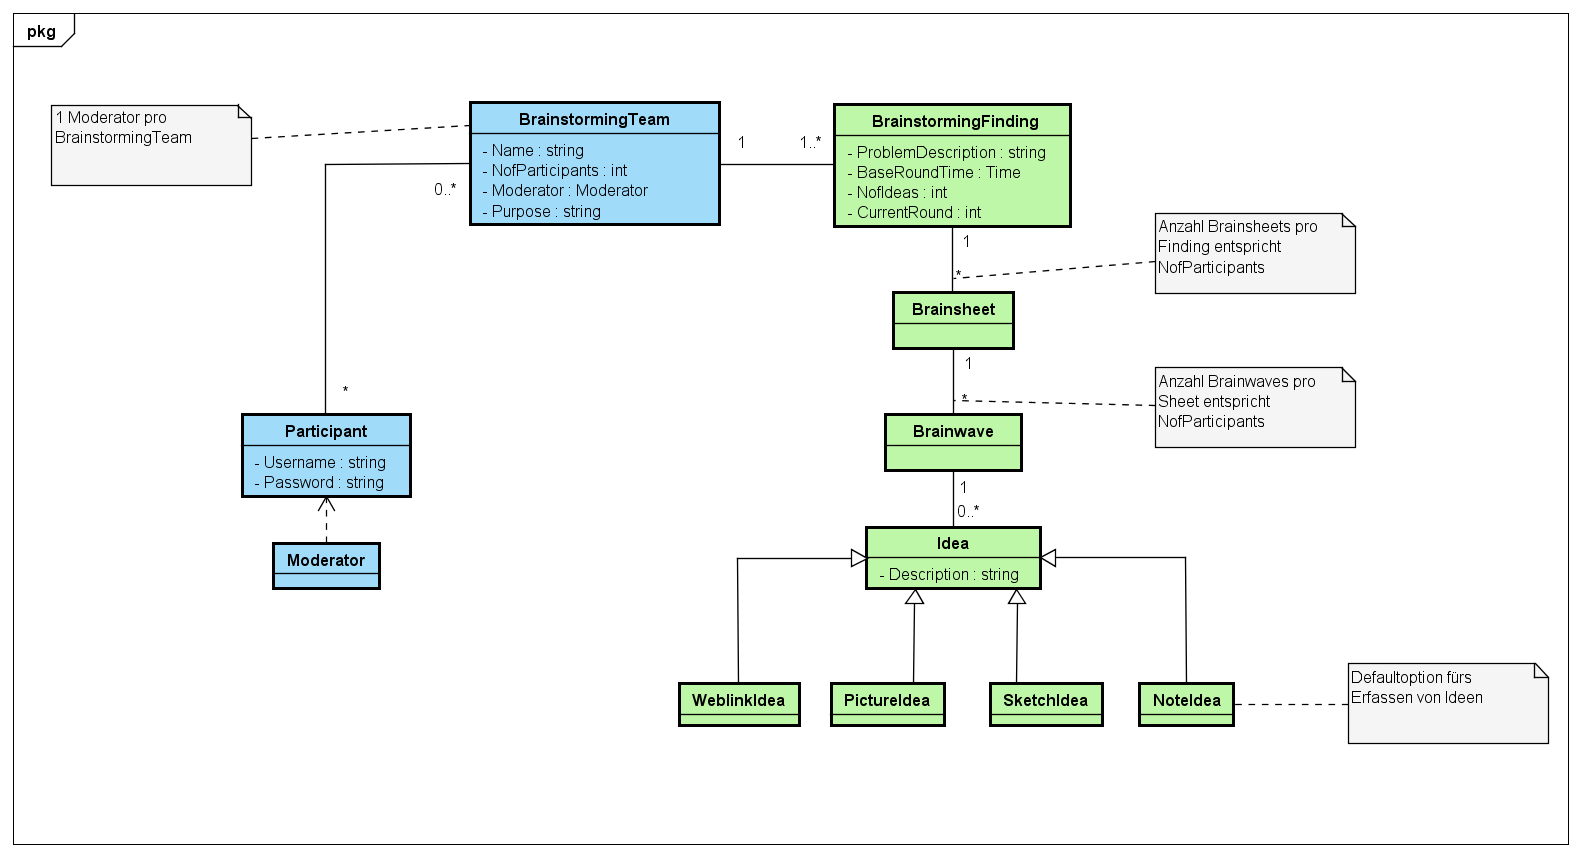
\includegraphics[width=1\linewidth]{img/domain-analyse/DomainModell-Methode635}
	\caption{Domain Modell BrainingOutOfBox}
	\label{fig:domainmodell-methode635}
\end{figure}
